\section{Timeline for project}
This semester project can be split into 6 parts, as seen on \autoref{fig:timeline-for-project}.
There are 4 sprints in total for development of the application. 
For the PO and process group there is a lot of work to prepare the first sprint.
This is what we consider \textit{Pre sprint 1}.
After this, there are 4 sprints to planned the week planner application.
The process group planned the sprints such that the last sprint will end two weeks before the deadline for handing in the project.
These last two weeks will be spent on usability tests with the customers and finishing the report.
What is common for every sprint is that they follow the scrum of scrum guidelines previously described in \autoref{scrum-of-scrums}.

\begin{figure}[H]
    \center{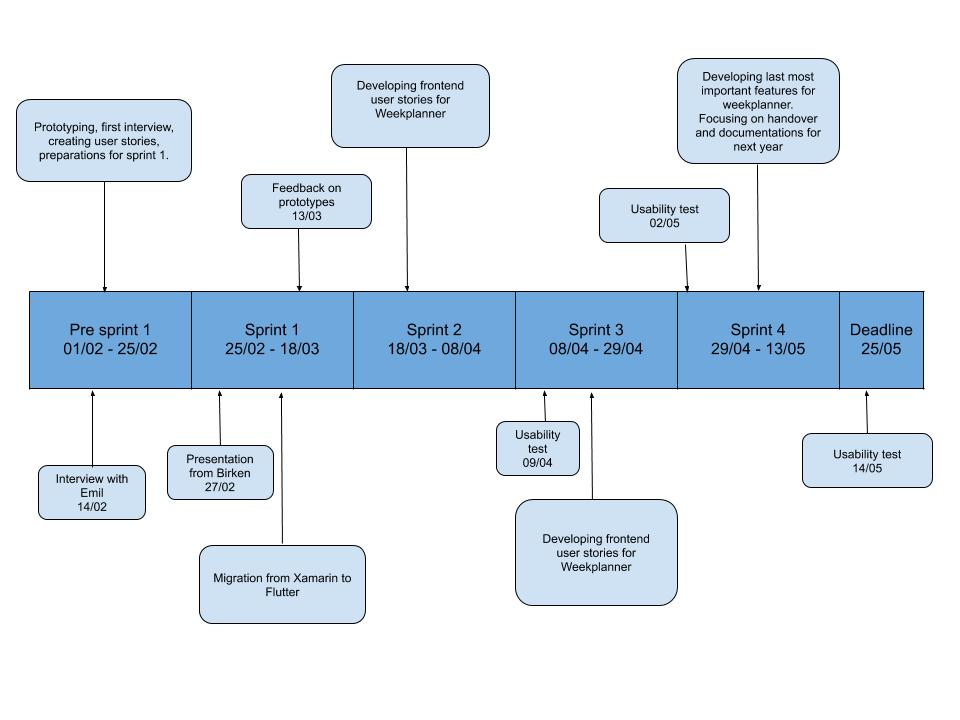
\includegraphics[width=\textwidth]
    {figures/timeline-for-entire-project.JPG}}
    \caption{\label{fig:timeline-for-project} Timeline for the project.}
\end{figure}

\todo{Figure is updated continously}

\subsubsection{Pre sprint 1}
\textit{Pre sprint 1} was where the preparation for the first sprint happened.
During this time, the groups of the GIRAF project did not fully understand the project, so it was mostly spent gathering information.
During this time the POs contact and interview customers to gain insight into what is wanted by the customers.
With these interviews, user stories and prototypes are created so that they are ready for sprint 1.
In \textit{pre sprint 1}, an interview with Emil from Egebakken was conducted. 
This interview is described in \autoref{interview-with-emil}.

\subsubsection{Sprint 1}
A presentation from the kindergarten Birken was given on February 27th.
This presentation is described in \autoref{presentation-from-birken}.
The focus of this sprint started out as fixing bugs and making the application more stable.
It turned out that there were a lot of problems with the frontend with Xamarin, and it was decided that the frontend should be migrated to Flutter during an extraordinary meeting involving most participants of the project. \\
The pros and cons of the decision are described in \autoref{change-of-framework}.
This also resulted in the PO group needing to look into the user stories, as new user stories for previously implemented features needed to be implemented again and many of the old user stories had to gain a lower priority.
A meeting was planned with the customers on March 13th to get feedback on the prototypes. 
This interview resulted in some of the prototypes getting reworked to better fit the customers needs.

\subsubsection{Sprint 2}
As there was no release at the end of sprint 1 because of the decision to migrate to flutter, no usability test could be conducted.
Instead this sprint was spent developing user stories planned in sprint 1.


\todo{To be continued...}

\subsubsection{Sprint 3}
\todo{Write in sprint 3}

\subsubsection{Sprint 4}
\todo{Write in sprint 4}
\subsubsection{Deadline}
\todo{Write after usability test after sprint 4.}
